
%(BEGIN_QUESTION)
% Copyright 2011, Tony R. Kuphaldt, released under the Creative Commons Attribution License (v 1.0)
% This means you may do almost anything with this work of mine, so long as you give me proper credit

A ``smart'' DP transmitter and orifice plate were recently installed to measure flow through a pipe.  The orifice plate range is 0 to 150 inches WC at 0 to 1000 gallons per minute:

$$\includegraphics[width=15.5cm]{i03428x01.eps}$$

Operations personnel register a flow rate of 699 gallons per minute on the display of their DCS, which they believe to be too much.  Based on what you see here, do you think there is a problem, or is this new system working as it should?

\underbar{file i03428}
%(END_QUESTION)





%(BEGIN_ANSWER)

The problem lies with the DCS: to be specific, someone has configured square-root characterization in it as well as within the transmitter!

%(END_ANSWER)





%(BEGIN_NOTES)


%INDEX% Calibration, smart transmitter: digital trim
%INDEX% Fieldbus, HART: communicator variables
%INDEX% Measurement, flow: square root characterized pressure transmitter

%(END_NOTES)

